\documentclass[10pt,a4paper]{article}
\usepackage[margin=2.3cm]{geometry}
\usepackage{graphicx}
\usepackage{booktabs}
\usepackage{amsmath,amssymb}
\usepackage[font=small,labelfont=bf]{caption}
\usepackage[hidelinks]{hyperref}
\usepackage{xcolor}
\usepackage{float}
\usepackage[round]{natbib}
\usepackage[section]{placeins}
\newcommand{\V}[1]{\ifcsname v:#1\endcsname\csname v:#1\endcsname\else\textbf{??#1}\GenericWarning{}{missing value #1}\fi}
\expandafter\def\csname v:geodW\endcsname{100}
\expandafter\def\csname v:bandM\endcsname{50}
\expandafter\def\csname v:profDz\endcsname{200}
\expandafter\def\csname v:profReg\endcsname{0.05}
\expandafter\def\csname v:smbUpd\endcsname{5}
\expandafter\def\csname v:geodLawB\endcsname{-0.18}
\expandafter\def\csname v:geodLawDh\endcsname{-0.57}
\expandafter\def\csname v:geodLawEps\endcsname{0.38}
\expandafter\def\csname v:geodLawNative\endcsname{-0.14}
\expandafter\def\csname v:geodBandB\endcsname{+0.37}
\expandafter\def\csname v:geodBandDh\endcsname{-0.05}
\expandafter\def\csname v:geodFinalB\endcsname{+0.02}
\expandafter\def\csname v:geodFinalDh\endcsname{-0.38}
\expandafter\def\csname v:geodEpsMin\endcsname{0.34}
\expandafter\def\csname v:geodEpsMax\endcsname{0.42}
\expandafter\def\csname v:scanJmin\endcsname{+0.27}
\expandafter\def\csname v:scanTmin\endcsname{0.00}
\expandafter\def\csname v:scanJzero\endcsname{7.97}
\expandafter\def\csname v:scanJbest\endcsname{7.51}
\expandafter\def\csname v:scanGstep\endcsname{1}
\expandafter\def\csname v:epsRealMax\endcsname{0.11}
\expandafter\def\csname v:epsGthree\endcsname{0.37}
\expandafter\def\csname v:epsStwo\endcsname{0.30}
\expandafter\def\csname v:epsSone\endcsname{0.39}
\expandafter\def\csname v:nogGthreeB\endcsname{-0.38}
\expandafter\def\csname v:nogGthreeObs\endcsname{-0.88}
\expandafter\def\csname v:nogStwoB\endcsname{-0.12}
\expandafter\def\csname v:nogStwoObs\endcsname{-0.42}
\expandafter\def\csname v:ablCellsRmse\endcsname{1.15}
\expandafter\def\csname v:ablCellsBias\endcsname{-0.15}
\expandafter\def\csname v:ablCellsEla\endcsname{2272}
\expandafter\def\csname v:ablCellsGRmse\endcsname{1.12}
\expandafter\def\csname v:ablCellsGBias\endcsname{-0.04}
\expandafter\def\csname v:ablCellsGEla\endcsname{2264}
\expandafter\def\csname v:ablBandsRmse\endcsname{0.71}
\expandafter\def\csname v:ablBandsBias\endcsname{+0.41}
\expandafter\def\csname v:ablBandsEla\endcsname{2318}
\expandafter\def\csname v:ablBandsGRmse\endcsname{0.60}
\expandafter\def\csname v:ablBandsGBias\endcsname{+0.04}
\expandafter\def\csname v:ablBandsGEla\endcsname{2335}
\expandafter\def\csname v:nogElaS01\endcsname{2318}
\expandafter\def\csname v:geodElaS01\endcsname{2335}
\expandafter\def\csname v:nogElaS02\endcsname{3150}
\expandafter\def\csname v:geodElaS02\endcsname{3183}
\expandafter\def\csname v:nogElaG03\endcsname{2871}
\expandafter\def\csname v:geodElaG03\endcsname{2890}
\expandafter\def\csname v:fldReg\endcsname{3}
\expandafter\def\csname v:fldNodes\endcsname{500}
\expandafter\def\csname v:fldN\endcsname{5}
\expandafter\def\csname v:fldCellProf\endcsname{11.7}
\expandafter\def\csname v:fldCellField\endcsname{8.3}
\expandafter\def\csname v:fldBandProf\endcsname{1.61}
\expandafter\def\csname v:fldBandField\endcsname{1.39}
\expandafter\def\csname v:fldGwProf\endcsname{-0.74}
\expandafter\def\csname v:fldGwField\endcsname{-0.71}
\expandafter\def\csname v:fldElaProf\endcsname{1351}
\expandafter\def\csname v:fldElaField\endcsname{1365}
\expandafter\def\csname v:fldUncProf\endcsname{1.15}
\expandafter\def\csname v:fldUncField\endcsname{0.83}
\expandafter\def\csname v:fldDhField\endcsname{-0.67}
\expandafter\def\csname v:fldDhObs\endcsname{-0.71}
\expandafter\def\csname v:fldDiffMax\endcsname{1.4}
\expandafter\def\csname v:nPairs\endcsname{96}
\expandafter\def\csname v:redMedFirst\endcsname{12}
\expandafter\def\csname v:itsMedFirst\endcsname{17}
\expandafter\def\csname v:nMemFirst\endcsname{478}
\expandafter\def\csname v:redMedFinal\endcsname{85}
\expandafter\def\csname v:itsMedFinal\endcsname{24}
\expandafter\def\csname v:nMemFinal\endcsname{478}
\expandafter\def\csname v:redBelowFiveFirst\endcsname{20}
\expandafter\def\csname v:redMinFinal\endcsname{24}
\expandafter\def\csname v:lossS01FirstA\endcsname{41.3}
\expandafter\def\csname v:lossS01FirstB\endcsname{39.8}
\expandafter\def\csname v:lossS01FinalA\endcsname{25.3}
\expandafter\def\csname v:lossS01FinalB\endcsname{8.8}
\expandafter\def\csname v:lossS02FirstA\endcsname{12.9}
\expandafter\def\csname v:lossS02FirstB\endcsname{11.0}
\expandafter\def\csname v:lossS02FinalA\endcsname{118.6}
\expandafter\def\csname v:lossS02FinalB\endcsname{3.9}
\expandafter\def\csname v:lossG03FirstA\endcsname{23.0}
\expandafter\def\csname v:lossG03FirstB\endcsname{21.8}
\expandafter\def\csname v:lossG03FinalA\endcsname{19.2}
\expandafter\def\csname v:lossG03FinalB\endcsname{9.1}
\expandafter\def\csname v:lossG05FirstA\endcsname{14.9}
\expandafter\def\csname v:lossG05FirstB\endcsname{12.4}
\expandafter\def\csname v:lossG05FinalA\endcsname{13.7}
\expandafter\def\csname v:lossG05FinalB\endcsname{3.2}
\expandafter\def\csname v:sOneFirst\endcsname{0.85}
\expandafter\def\csname v:sOneFinal\endcsname{0.60}
\expandafter\def\csname v:sOneBetter\endcsname{12}
\expandafter\def\csname v:sOneN\endcsname{14}
\expandafter\def\csname v:sOneWorse\endcsname{EXP05}
\expandafter\def\csname v:sOneE05First\endcsname{0.66}
\expandafter\def\csname v:sOneE05Final\endcsname{2.19}
\expandafter\def\csname v:sOneE09First\endcsname{1.54}
\expandafter\def\csname v:sOneE09Final\endcsname{1.08}
\expandafter\def\csname v:sOneE12First\endcsname{1.41}
\expandafter\def\csname v:sOneE12Final\endcsname{0.91}
\expandafter\def\csname v:sOneE13First\endcsname{0.68}
\expandafter\def\csname v:sOneE13Final\endcsname{0.67}
\expandafter\def\csname v:sOneE14First\endcsname{1.36}
\expandafter\def\csname v:sOneE14Final\endcsname{0.88}
\expandafter\def\csname v:sOneE15First\endcsname{27.6}
\expandafter\def\csname v:sOneE15Final\endcsname{4.7}
\expandafter\def\csname v:sOneRegMin\endcsname{0.59}
\expandafter\def\csname v:sOneRegMax\endcsname{1.08}
\expandafter\def\csname v:sOnePixFinal\endcsname{0.57}
\expandafter\def\csname v:sOnePixFirst\endcsname{0.67}
\expandafter\def\csname v:sOneRtwo\endcsname{0.96}
\expandafter\def\csname v:sOneRtwoFirst\endcsname{0.95}
\expandafter\def\csname v:sOneElaLo\endcsname{2324}
\expandafter\def\csname v:sOneElaHi\endcsname{2346}
\expandafter\def\csname v:sOneElaFirstLo\endcsname{2277}
\expandafter\def\csname v:sOneElaFirstHi\endcsname{2284}
\expandafter\def\csname v:sOneGw\endcsname{+0.06}
\expandafter\def\csname v:sOneGwTrue\endcsname{-0.14}
\expandafter\def\csname v:sOneGwFirst\endcsname{-0.00}
\expandafter\def\csname v:sOneDhMod\endcsname{-0.32}
\expandafter\def\csname v:sOneDhModFirst\endcsname{-0.90}
\expandafter\def\csname v:sOneFdivRmse\endcsname{2.9}
\expandafter\def\csname v:sOneFdivRmseFirst\endcsname{4.1}
\expandafter\def\csname v:sOneThk\endcsname{98}
\expandafter\def\csname v:sOneThkTrue\endcsname{54}
\expandafter\def\csname v:sTwoGwFirst\endcsname{-0.17}
\expandafter\def\csname v:sTwoGw\endcsname{-0.39}
\expandafter\def\csname v:sTwoDhMod\endcsname{-0.68}
\expandafter\def\csname v:sTwoDhObs\endcsname{-0.42}
\expandafter\def\csname v:sTwoThkBias\endcsname{+14}
\expandafter\def\csname v:sTwoThkRmse\endcsname{51}
\expandafter\def\csname v:sTwoThkR\endcsname{0.97}
\expandafter\def\csname v:sTwoEla\endcsname{3183}
\expandafter\def\csname v:sTwoGwMin\endcsname{-0.42}
\expandafter\def\csname v:sTwoGwMax\endcsname{-0.39}
\expandafter\def\csname v:sTwoGwFourteen\endcsname{-0.39}
\expandafter\def\csname v:sTwoElaE02\endcsname{2704}
\expandafter\def\csname v:sTwoElaE13\endcsname{3321}
\expandafter\def\csname v:sTwoElaE14\endcsname{3258}
\expandafter\def\csname v:sTwoThkRmseRaw\endcsname{93}
\expandafter\def\csname v:gwG01\endcsname{-0.74}
\expandafter\def\csname v:elaG01\endcsname{1351}
\expandafter\def\csname v:dhModG01\endcsname{-0.68}
\expandafter\def\csname v:dhObsG01\endcsname{-0.71}
\expandafter\def\csname v:fdivG01\endcsname{-0.06}
\expandafter\def\csname v:uncG01\endcsname{1.15}
\expandafter\def\csname v:thkG01\endcsname{147}
\expandafter\def\csname v:gwG02\endcsname{+1.30}
\expandafter\def\csname v:elaG02\endcsname{5118}
\expandafter\def\csname v:dhModG02\endcsname{+1.32}
\expandafter\def\csname v:dhObsG02\endcsname{+1.64}
\expandafter\def\csname v:fdivG02\endcsname{-0.02}
\expandafter\def\csname v:uncG02\endcsname{1.12}
\expandafter\def\csname v:thkG02\endcsname{34}
\expandafter\def\csname v:gprTestG02\endcsname{14}
\expandafter\def\csname v:gwG03\endcsname{-0.89}
\expandafter\def\csname v:elaG03\endcsname{2890}
\expandafter\def\csname v:dhModG03\endcsname{-1.23}
\expandafter\def\csname v:dhObsG03\endcsname{-0.88}
\expandafter\def\csname v:fdivG03\endcsname{+0.34}
\expandafter\def\csname v:uncG03\endcsname{2.59}
\expandafter\def\csname v:thkG03\endcsname{140}
\expandafter\def\csname v:gprTestG03\endcsname{51}
\expandafter\def\csname v:gwG04\endcsname{-1.31}
\expandafter\def\csname v:elaG04\endcsname{4684}
\expandafter\def\csname v:dhModG04\endcsname{-1.19}
\expandafter\def\csname v:dhObsG04\endcsname{-1.30}
\expandafter\def\csname v:fdivG04\endcsname{-0.12}
\expandafter\def\csname v:uncG04\endcsname{0.51}
\expandafter\def\csname v:thkG04\endcsname{28}
\expandafter\def\csname v:gwG05\endcsname{-2.01}
\expandafter\def\csname v:elaG05\endcsname{3191}
\expandafter\def\csname v:dhModG05\endcsname{-1.98}
\expandafter\def\csname v:dhObsG05\endcsname{-1.95}
\expandafter\def\csname v:fdivG05\endcsname{-0.03}
\expandafter\def\csname v:uncG05\endcsname{2.02}
\expandafter\def\csname v:thkG05\endcsname{161}
\expandafter\def\csname v:gprTestG05\endcsname{65}
\expandafter\def\csname v:gwG06\endcsname{-1.01}
\expandafter\def\csname v:elaG06\endcsname{3126}
\expandafter\def\csname v:dhModG06\endcsname{-0.95}
\expandafter\def\csname v:dhObsG06\endcsname{-0.96}
\expandafter\def\csname v:fdivG06\endcsname{-0.06}
\expandafter\def\csname v:uncG06\endcsname{1.68}
\expandafter\def\csname v:thkG06\endcsname{117}
\expandafter\def\csname v:famSpreadMax\endcsname{0.06}
\expandafter\def\csname v:closMax\endcsname{0.35}
\expandafter\def\csname v:uncMin\endcsname{0.5}
\expandafter\def\csname v:uncMax\endcsname{2.6}
\expandafter\def\csname v:dSmbMaxG01\endcsname{0.01}
\expandafter\def\csname v:dElaMaxG01\endcsname{9}
\expandafter\def\csname v:dElaMaxExpG01\endcsname{EXP13}
\expandafter\def\csname v:dSmbMaxNoResG01\endcsname{0.00}
\expandafter\def\csname v:dElaMaxNoResG01\endcsname{9}
\expandafter\def\csname v:gwG01EXP15\endcsname{-0.73}
\expandafter\def\csname v:dhG01EXP15\endcsname{-0.70}
\expandafter\def\csname v:rawGwG01\endcsname{-0.75}
\expandafter\def\csname v:rawElaG01\endcsname{0}
\expandafter\def\csname v:dSmbMaxG05\endcsname{0.22}
\expandafter\def\csname v:dElaMaxG05\endcsname{16}
\expandafter\def\csname v:dElaMaxExpG05\endcsname{EXP13}
\expandafter\def\csname v:dSmbMaxNoResG05\endcsname{0.00}
\expandafter\def\csname v:dElaMaxNoResG05\endcsname{16}
\expandafter\def\csname v:gwG05EXP14\endcsname{-1.94}
\expandafter\def\csname v:dhG05EXP14\endcsname{-1.90}
\expandafter\def\csname v:gwG05EXP15\endcsname{-1.80}
\expandafter\def\csname v:dhG05EXP15\endcsname{-1.76}
\expandafter\def\csname v:rawGwG05\endcsname{-2.00}
\expandafter\def\csname v:rawElaG05\endcsname{9}
\expandafter\def\csname v:respS02E03\endcsname{0.04}
\expandafter\def\csname v:respS02E04\endcsname{0.05}
\expandafter\def\csname v:respS02E05\endcsname{0.09}
\expandafter\def\csname v:respS02E06\endcsname{0.06}
\expandafter\def\csname v:respS02E07\endcsname{0.06}
\expandafter\def\csname v:respS02E08\endcsname{0.07}
\expandafter\def\csname v:respS02E09\endcsname{0.73}
\expandafter\def\csname v:respS02E10\endcsname{0.12}
\expandafter\def\csname v:respS02E11\endcsname{0.05}
\expandafter\def\csname v:respS02E12\endcsname{0.37}
\expandafter\def\csname v:respS02E13\endcsname{2.49}
\expandafter\def\csname v:respS02E15\endcsname{0.02}
\expandafter\def\csname v:respS02E14\endcsname{1.56}
\expandafter\def\csname v:respS02E02\endcsname{2.47}
\expandafter\def\csname v:respG01E03\endcsname{0.05}
\expandafter\def\csname v:respG01E04\endcsname{0.04}
\expandafter\def\csname v:respG01E05\endcsname{0.04}
\expandafter\def\csname v:respG01E06\endcsname{0.05}
\expandafter\def\csname v:respG01E07\endcsname{0.04}
\expandafter\def\csname v:respG01E08\endcsname{0.04}
\expandafter\def\csname v:respG01E09\endcsname{0.04}
\expandafter\def\csname v:respG01E10\endcsname{0.05}
\expandafter\def\csname v:respG01E11\endcsname{0.02}
\expandafter\def\csname v:respG01E12\endcsname{0.05}
\expandafter\def\csname v:respG01E13\endcsname{0.17}
\expandafter\def\csname v:respG01E15\endcsname{0.06}
\expandafter\def\csname v:respG01E02\endcsname{0.04}
\expandafter\def\csname v:respG05E03\endcsname{0.23}
\expandafter\def\csname v:respG05E04\endcsname{0.28}
\expandafter\def\csname v:respG05E05\endcsname{0.04}
\expandafter\def\csname v:respG05E06\endcsname{0.02}
\expandafter\def\csname v:respG05E07\endcsname{0.23}
\expandafter\def\csname v:respG05E08\endcsname{0.09}
\expandafter\def\csname v:respG05E09\endcsname{0.12}
\expandafter\def\csname v:respG05E10\endcsname{0.06}
\expandafter\def\csname v:respG05E11\endcsname{0.06}
\expandafter\def\csname v:respG05E12\endcsname{0.12}
\expandafter\def\csname v:respG05E13\endcsname{0.14}
\expandafter\def\csname v:respG05E15\endcsname{0.75}
\expandafter\def\csname v:respG05E14\endcsname{0.28}
\expandafter\def\csname v:respG05E02\endcsname{0.16}
\expandafter\def\csname v:respThkMaxS02\endcsname{0.09}
\expandafter\def\csname v:respVelMaxS02\endcsname{2.49}
\expandafter\def\csname v:respThkMaxG01\endcsname{0.05}
\expandafter\def\csname v:respVelMaxG01\endcsname{0.17}
\expandafter\def\csname v:respThkMaxG05\endcsname{0.28}
\expandafter\def\csname v:respVelMaxG05\endcsname{0.14}
\expandafter\def\csname v:repeatFloor\endcsname{0.05}
\expandafter\def\csname v:glG01E01\endcsname{-0.74}
\expandafter\def\csname v:glElaG01E01\endcsname{1351}
\expandafter\def\csname v:glDhG01E01\endcsname{-0.71}
\expandafter\def\csname v:glThkG01E01\endcsname{147}
\expandafter\def\csname v:glG01E02\endcsname{-0.75}
\expandafter\def\csname v:glElaG01E02\endcsname{1350}
\expandafter\def\csname v:glDhG01E02\endcsname{-0.73}
\expandafter\def\csname v:glThkG01E02\endcsname{144}
\expandafter\def\csname v:glG01E16\endcsname{-0.97}
\expandafter\def\csname v:glElaG01E16\endcsname{1367}
\expandafter\def\csname v:glDhG01E16\endcsname{-0.94}
\expandafter\def\csname v:glThkG01E16\endcsname{207}
\expandafter\def\csname v:glG01E17\endcsname{-0.96}
\expandafter\def\csname v:glElaG01E17\endcsname{1392}
\expandafter\def\csname v:glDhG01E17\endcsname{-0.94}
\expandafter\def\csname v:glThkG01E17\endcsname{143}
\expandafter\def\csname v:glG01E18\endcsname{-0.96}
\expandafter\def\csname v:glElaG01E18\endcsname{1392}
\expandafter\def\csname v:glDhG01E18\endcsname{-0.94}
\expandafter\def\csname v:glThkG01E18\endcsname{143}
\expandafter\def\csname v:glG01E19\endcsname{-0.96}
\expandafter\def\csname v:glElaG01E19\endcsname{1392}
\expandafter\def\csname v:glDhG01E19\endcsname{-0.94}
\expandafter\def\csname v:glThkG01E19\endcsname{143}
\expandafter\def\csname v:glG01E20\endcsname{-0.97}
\expandafter\def\csname v:glElaG01E20\endcsname{1357}
\expandafter\def\csname v:glDhG01E20\endcsname{-0.94}
\expandafter\def\csname v:glThkG01E20\endcsname{240}
\expandafter\def\csname v:glG02E01\endcsname{+1.30}
\expandafter\def\csname v:glElaG02E01\endcsname{5118}
\expandafter\def\csname v:glDhG02E01\endcsname{+1.64}
\expandafter\def\csname v:glThkG02E01\endcsname{34}
\expandafter\def\csname v:glG02E02\endcsname{+1.23}
\expandafter\def\csname v:glElaG02E02\endcsname{5116}
\expandafter\def\csname v:glDhG02E02\endcsname{+1.62}
\expandafter\def\csname v:glThkG02E02\endcsname{28}
\expandafter\def\csname v:glG02E16\endcsname{-0.51}
\expandafter\def\csname v:glElaG02E16\endcsname{5436}
\expandafter\def\csname v:glDhG02E16\endcsname{-0.49}
\expandafter\def\csname v:glThkG02E16\endcsname{34}
\expandafter\def\csname v:glG02E17\endcsname{-0.51}
\expandafter\def\csname v:glElaG02E17\endcsname{5424}
\expandafter\def\csname v:glDhG02E17\endcsname{-0.49}
\expandafter\def\csname v:glThkG02E17\endcsname{23}
\expandafter\def\csname v:glG02E18\endcsname{-0.51}
\expandafter\def\csname v:glElaG02E18\endcsname{5425}
\expandafter\def\csname v:glDhG02E18\endcsname{-0.49}
\expandafter\def\csname v:glThkG02E18\endcsname{23}
\expandafter\def\csname v:glG02E19\endcsname{-0.51}
\expandafter\def\csname v:glElaG02E19\endcsname{5437}
\expandafter\def\csname v:glDhG02E19\endcsname{-0.49}
\expandafter\def\csname v:glThkG02E19\endcsname{33}
\expandafter\def\csname v:glG02E20\endcsname{-0.51}
\expandafter\def\csname v:glElaG02E20\endcsname{5436}
\expandafter\def\csname v:glDhG02E20\endcsname{-0.49}
\expandafter\def\csname v:glThkG02E20\endcsname{33}
\expandafter\def\csname v:glG03E01\endcsname{-0.89}
\expandafter\def\csname v:glElaG03E01\endcsname{2890}
\expandafter\def\csname v:glDhG03E01\endcsname{-0.88}
\expandafter\def\csname v:glThkG03E01\endcsname{140}
\expandafter\def\csname v:glG03E02\endcsname{-0.88}
\expandafter\def\csname v:glElaG03E02\endcsname{2879}
\expandafter\def\csname v:glDhG03E02\endcsname{-0.87}
\expandafter\def\csname v:glThkG03E02\endcsname{130}
\expandafter\def\csname v:glG03E16\endcsname{-1.09}
\expandafter\def\csname v:glElaG03E16\endcsname{2964}
\expandafter\def\csname v:glDhG03E16\endcsname{-1.06}
\expandafter\def\csname v:glThkG03E16\endcsname{95}
\expandafter\def\csname v:glG03E17\endcsname{-1.12}
\expandafter\def\csname v:glElaG03E17\endcsname{2920}
\expandafter\def\csname v:glDhG03E17\endcsname{-1.06}
\expandafter\def\csname v:glThkG03E17\endcsname{130}
\expandafter\def\csname v:glG03E18\endcsname{-1.12}
\expandafter\def\csname v:glElaG03E18\endcsname{2920}
\expandafter\def\csname v:glDhG03E18\endcsname{-1.06}
\expandafter\def\csname v:glThkG03E18\endcsname{130}
\expandafter\def\csname v:glG03E19\endcsname{-1.12}
\expandafter\def\csname v:glElaG03E19\endcsname{2920}
\expandafter\def\csname v:glDhG03E19\endcsname{-1.06}
\expandafter\def\csname v:glThkG03E19\endcsname{130}
\expandafter\def\csname v:glG03E20\endcsname{-1.09}
\expandafter\def\csname v:glElaG03E20\endcsname{2993}
\expandafter\def\csname v:glDhG03E20\endcsname{-1.06}
\expandafter\def\csname v:glThkG03E20\endcsname{69}
\expandafter\def\csname v:glG04E01\endcsname{-1.31}
\expandafter\def\csname v:glElaG04E01\endcsname{4684}
\expandafter\def\csname v:glDhG04E01\endcsname{-1.30}
\expandafter\def\csname v:glThkG04E01\endcsname{28}
\expandafter\def\csname v:glG04E02\endcsname{-1.31}
\expandafter\def\csname v:glElaG04E02\endcsname{4673}
\expandafter\def\csname v:glDhG04E02\endcsname{-1.30}
\expandafter\def\csname v:glThkG04E02\endcsname{9}
\expandafter\def\csname v:glG04E16\endcsname{-0.43}
\expandafter\def\csname v:glElaG04E16\endcsname{4696}
\expandafter\def\csname v:glDhG04E16\endcsname{-0.42}
\expandafter\def\csname v:glThkG04E16\endcsname{12}
\expandafter\def\csname v:glG04E17\endcsname{-0.43}
\expandafter\def\csname v:glElaG04E17\endcsname{--}
\expandafter\def\csname v:glDhG04E17\endcsname{-0.42}
\expandafter\def\csname v:glThkG04E17\endcsname{28}
\expandafter\def\csname v:glG04E18\endcsname{-0.43}
\expandafter\def\csname v:glElaG04E18\endcsname{--}
\expandafter\def\csname v:glDhG04E18\endcsname{-0.42}
\expandafter\def\csname v:glThkG04E18\endcsname{28}
\expandafter\def\csname v:glG04E19\endcsname{-0.43}
\expandafter\def\csname v:glElaG04E19\endcsname{--}
\expandafter\def\csname v:glDhG04E19\endcsname{-0.42}
\expandafter\def\csname v:glThkG04E19\endcsname{28}
\expandafter\def\csname v:glG04E20\endcsname{-0.43}
\expandafter\def\csname v:glElaG04E20\endcsname{4697}
\expandafter\def\csname v:glDhG04E20\endcsname{-0.42}
\expandafter\def\csname v:glThkG04E20\endcsname{12}
\expandafter\def\csname v:glG05E01\endcsname{-2.01}
\expandafter\def\csname v:glElaG05E01\endcsname{3191}
\expandafter\def\csname v:glDhG05E01\endcsname{-1.95}
\expandafter\def\csname v:glThkG05E01\endcsname{161}
\expandafter\def\csname v:glG05E02\endcsname{-2.00}
\expandafter\def\csname v:glElaG05E02\endcsname{3182}
\expandafter\def\csname v:glDhG05E02\endcsname{-1.95}
\expandafter\def\csname v:glThkG05E02\endcsname{159}
\expandafter\def\csname v:glG05E16\endcsname{-1.32}
\expandafter\def\csname v:glElaG05E16\endcsname{3212}
\expandafter\def\csname v:glDhG05E16\endcsname{-1.29}
\expandafter\def\csname v:glThkG05E16\endcsname{171}
\expandafter\def\csname v:glG05E17\endcsname{-1.32}
\expandafter\def\csname v:glElaG05E17\endcsname{3128}
\expandafter\def\csname v:glDhG05E17\endcsname{-1.29}
\expandafter\def\csname v:glThkG05E17\endcsname{169}
\expandafter\def\csname v:glG05E18\endcsname{-1.32}
\expandafter\def\csname v:glElaG05E18\endcsname{3129}
\expandafter\def\csname v:glDhG05E18\endcsname{-1.29}
\expandafter\def\csname v:glThkG05E18\endcsname{169}
\expandafter\def\csname v:glG05E19\endcsname{-1.32}
\expandafter\def\csname v:glElaG05E19\endcsname{3129}
\expandafter\def\csname v:glDhG05E19\endcsname{-1.29}
\expandafter\def\csname v:glThkG05E19\endcsname{169}
\expandafter\def\csname v:glG05E20\endcsname{-1.32}
\expandafter\def\csname v:glElaG05E20\endcsname{3218}
\expandafter\def\csname v:glDhG05E20\endcsname{-1.29}
\expandafter\def\csname v:glThkG05E20\endcsname{180}
\expandafter\def\csname v:glG06E01\endcsname{-1.01}
\expandafter\def\csname v:glElaG06E01\endcsname{3126}
\expandafter\def\csname v:glDhG06E01\endcsname{-0.96}
\expandafter\def\csname v:glThkG06E01\endcsname{117}
\expandafter\def\csname v:glG06E02\endcsname{-1.00}
\expandafter\def\csname v:glElaG06E02\endcsname{3109}
\expandafter\def\csname v:glDhG06E02\endcsname{-0.95}
\expandafter\def\csname v:glThkG06E02\endcsname{90}
\expandafter\def\csname v:glG06E16\endcsname{-0.82}
\expandafter\def\csname v:glElaG06E16\endcsname{--}
\expandafter\def\csname v:glDhG06E16\endcsname{-0.79}
\expandafter\def\csname v:glThkG06E16\endcsname{54}
\expandafter\def\csname v:glG06E17\endcsname{-0.83}
\expandafter\def\csname v:glElaG06E17\endcsname{3103}
\expandafter\def\csname v:glDhG06E17\endcsname{-0.79}
\expandafter\def\csname v:glThkG06E17\endcsname{92}
\expandafter\def\csname v:glG06E18\endcsname{-0.82}
\expandafter\def\csname v:glElaG06E18\endcsname{3113}
\expandafter\def\csname v:glDhG06E18\endcsname{-0.79}
\expandafter\def\csname v:glThkG06E18\endcsname{118}
\expandafter\def\csname v:glG06E19\endcsname{-0.82}
\expandafter\def\csname v:glElaG06E19\endcsname{3116}
\expandafter\def\csname v:glDhG06E19\endcsname{-0.79}
\expandafter\def\csname v:glThkG06E19\endcsname{117}
\expandafter\def\csname v:glG06E20\endcsname{-0.82}
\expandafter\def\csname v:glElaG06E20\endcsname{--}
\expandafter\def\csname v:glDhG06E20\endcsname{-0.79}
\expandafter\def\csname v:glThkG06E20\endcsname{54}
\expandafter\def\csname v:rawGwMax\endcsname{0.07}
\expandafter\def\csname v:rawElaMax\endcsname{17}
\expandafter\def\csname v:idGwMax\endcsname{0.00}
\expandafter\def\csname v:idElaMax\endcsname{13}
\expandafter\def\csname v:idThkMax\endcsname{34}
\expandafter\def\csname v:uncRatioMin\endcsname{0.8}
\expandafter\def\csname v:uncRatioMax\endcsname{4.0}

\setlength{\parskip}{3pt}
\renewcommand{\topfraction}{0.9}\renewcommand{\bottomfraction}{0.8}\renewcommand{\textfraction}{0.07}\renewcommand{\floatpagefraction}{0.8}
\renewcommand{\arraystretch}{1.12}
\newcommand{\myr}{m\,yr$^{-1}$}
\newcommand{\mie}{m\,i.e.\,yr$^{-1}$}
\graphicspath{{figures_final/}}

\title{\textbf{Transient surface-mass-balance inversion with IGM\\for the ContinuIX intercomparison}\\[4pt]
\large Results (GROUP\_UNIL, method01)}
\author{Kejdi Lleshi\\ \small Institute of Earth Surface Dynamics, University of Lausanne}
\date{\small Working document, 28 October 2026}

\begin{document}
\maketitle

%=====================================================================================================================
\section{Setup}
ContinuIX compares methods that derive the surface mass balance (SMB) from the continuity equation
\citep{continuix}. Table~\ref{tab:exp} lists the twenty experiments and Table~\ref{tab:glaciers} the eight glaciers.
Our method runs in two steps, with the same automatic settings for every glacier--experiment pair:
a data assimilation (DA) that gives the ice thickness and the bed, and an SMB inference on that geometry.
\V{nPairs} of the 97 mandatory runs are complete. EXP14 for G01 (75\,m grid) does not fit into the memory of one GPU.

\subsection{Data assimilation}
The ice thickness $H_{\rm DA}$, and with it the bed $B=s_{\rm DA}-H_{\rm DA}$, is inverted from the surface velocities, and
from radar (GPR) thickness profiles where they exist, through the convolutional ice-flow emulator of IGM \citep{igm}. No
provided thickness or bed field is used. Up to five sliding coefficients $\tau$ fit the velocities equally well. Each of
these family members goes through the SMB inference, and SMB and flux divergence (FDIV) are reported as the family mean.

\subsection{SMB inference}
The SMB is found by differentiating a transient forward run over the observation window $t_1$--$t_2$,
$\Delta t=t_2-t_1$ \citep{lleshi}. The run starts from the observed surface on the assimilated bed,
$H(t_1)=\max(s_{\rm obs}(t_1)-B,\,0)$ on the ice mask $\Omega$, and solves the continuity equation
\begin{equation}
\frac{\partial H}{\partial t} = b - \nabla\cdot\left(H\,\bar{\mathbf u}\right),\qquad
\bar{\mathbf u}=\mathcal N(H,\,s,\,A,\,\tau),
\label{eq:cont}
\end{equation}
where $\bar{\mathbf u}$ is the depth-averaged velocity from the emulator $\mathcal N$ and $s=B+H$ is the surface. The time
step is fixed by the CFL condition of the initial state. The SMB is a piecewise-linear function of the surface elevation,
$b(z)=\sum_k b_k\,\phi_k(z)$, with hat functions $\phi_k$ on nodes \V{profDz}\,m apart. It is re-evaluated on the evolving
surface every \V{smbUpd}\,yr. Outside $\Omega$, $b=-10$\,\mie, so ice that flows across the outline melts. The node values
$\mathbf b$ minimise, with L-BFGS,
\begin{equation}
\mathcal L(\mathbf b) = J(\mathbf b)
 + \lambda\sum_k\left(b_{k-1}-2b_k+b_{k+1}\right)^2
 + w_g\left(\langle b\rangle - \dot h_{\rm obs}\right)^2 ,
\label{eq:loss}
\end{equation}
with $\lambda=\V{profReg}$ and $w_g=\V{geodW}$\,m$^{-1}$\,yr$^2$. The data term $J$ compares the simulated thickness at
$t_2$ with the observed one, $H_{\rm obs}(t_2)=s_{\rm obs}(t_2)-B$, after averaging in \V{bandM}\,m elevation bands $j$
of the window-start surface:
\begin{equation}
J = \left(\frac{\sum_j n_j\,\bar r_j^{\,2}}{\sum_j n_j}\right)^{1/2},\qquad
\bar r_j = \frac{1}{n_j}\sum_{i\in j}\left(H_i(t_2)-H_{{\rm obs},i}(t_2)\right),
\label{eq:band}
\end{equation}
where $n_j$ is the number of ice cells in band $j$. A profile $b(z)$ can only change the total thickness change in each
band. How ice is redistributed within a band depends on the DA thickness and is not fitted. In the last term,
$\langle\cdot\rangle$ is the mean over $\Omega$, with $b$ evaluated on the surface at $t_1$, and
$\dot h_{\rm obs}=\langle s_{\rm obs}(t_2)-s_{\rm obs}(t_1)\rangle/\Delta t$ is the observed glacier-wide elevation change.

\subsection{The geodetic term}
\label{sec:geod}
Integrating Eq.~(\ref{eq:cont}) over $\Omega$ gives
\begin{equation}
\left\langle\frac{\partial H}{\partial t}\right\rangle = \langle b\rangle
 - \frac{1}{|\Omega|}\oint_{\partial\Omega} H\,\bar{\mathbf u}\cdot\mathbf n\,{\rm d}l .
\label{eq:budget}
\end{equation}
Suppose $\Omega$ contains all the ice and no ice leaves it, as for a land-terminating glacier. Then the boundary flux
vanishes. Since the bed does not change, the glacier-wide SMB equals the observed mean elevation change,
$\langle b\rangle=\dot h_{\rm obs}$. This identity does not depend on the thickness, the bed or the ice flow; the
geodetic term in Eq.~(\ref{eq:loss}) imposes it.

The forward model does not conserve mass on $\Omega$ exactly. We define its budget error
\begin{equation}
\varepsilon = \langle b\rangle - \frac{\langle H(t_2)-H(t_1)\rangle}{\Delta t}.
\label{eq:eps}
\end{equation}
It is positive when the model moves ice across the outline, where it melts, and negative when clipping the thickness at
zero adds ice. It comes from the DA geometry and the emulator, not from the SMB. Since
$\langle H_{\rm obs}(t_2)-H(t_1)\rangle=\Delta t\,\dot h_{\rm obs}$, the mean thickness residual at $t_2$ is
\begin{equation}
\left\langle H(t_2)-H_{\rm obs}(t_2)\right\rangle = \Delta t\left(\langle b\rangle - \varepsilon - \dot h_{\rm obs}\right),
\label{eq:meanres}
\end{equation}
and by the Cauchy--Schwarz inequality $J$ cannot be smaller than the magnitude of this mean (up to the soft weighting of
margin cells). The band misfit alone is therefore smallest near $\langle b\rangle=\dot h_{\rm obs}+\varepsilon$: it
compensates the budget error of the model with a uniform SMB offset. The geodetic term instead pins $\langle b\rangle$ to
the observation. The budget error then stays in the thickness misfit and is attributed to the dynamics, where it
arises. With $w_g=\V{geodW}$, an offset of 0.1\,\mie\ adds \V{scanGstep}\,m to the loss, while $J$ changes by only a few
decimetres per 0.1\,\mie\ (Fig.~\ref{fig:geodmech}b). The term thus acts almost as a hard constraint on the
glacier-wide SMB and leaves the shape of the profile to $J$.

S01, a steady-state glacier with a prescribed SMB law, shows this mechanism (Fig.~\ref{fig:geodmech}):
\begin{itemize}\setlength{\itemsep}{1pt}
\item \textbf{The model loses ice even under the true SMB.} Driven by the prescribed law, whose mean over $\Omega$ is
$\V{geodLawB}$\,\mie, the model thins by $\V{geodLawDh}$\,\myr, although the observed change is zero:
$\varepsilon=\V{geodLawEps}$\,\mie. Every inversion gives a similar $\varepsilon$ (\V{geodEpsMin}--\V{geodEpsMax}).
\item \textbf{Without the geodetic term the SMB absorbs it.} The band misfit raises the profile until the modelled mean
thinning nearly vanishes ($\V{geodBandDh}$\,\myr), which takes $\langle b\rangle=\V{geodBandB}$\,\mie. Along a uniform
offset $\delta$ of the final profile, $J$ is smallest at $\delta=\V{scanJmin}$\,\mie\
(\V{scanJbest}\,m against \V{scanJzero}\,m at $\delta=0$). The full loss is smallest at $\delta=\V{scanTmin}$.
\item \textbf{With it the SMB keeps the observed budget.} $\langle b\rangle=\V{geodFinalB}$\,\mie, and the modelled
thinning of $\V{geodFinalDh}$\,\myr\ is left as thickness misfit.
\end{itemize}
On the real glaciers the budget error is small ($|\varepsilon|\le\V{epsRealMax}$\,\mie) except on G03
($\varepsilon=\V{epsGthree}$), whose terminus reaches the domain edge. On the synthetic S02 it is \V{epsStwo}. Without the
geodetic term, the glacier-wide SMB moves away from the observed change by about $\varepsilon$
(Fig.~\ref{fig:geodmech}c). On G03 it is $\V{nogGthreeB}$ instead of $\V{nogGthreeObs}$\,\mie, and the ELA is lowered
from \V{geodElaG03} to \V{nogElaG03}\,m. On S02 it is $\V{nogStwoB}$ instead of $\V{nogStwoObs}$, and the ELA is lowered
from \V{geodElaS02} to \V{nogElaS02}\,m. Because Eq.~(\ref{eq:budget}) requires $\langle b\rangle=\dot h_{\rm obs}$,
these shifts are errors.

\begin{figure}[H]
\centering
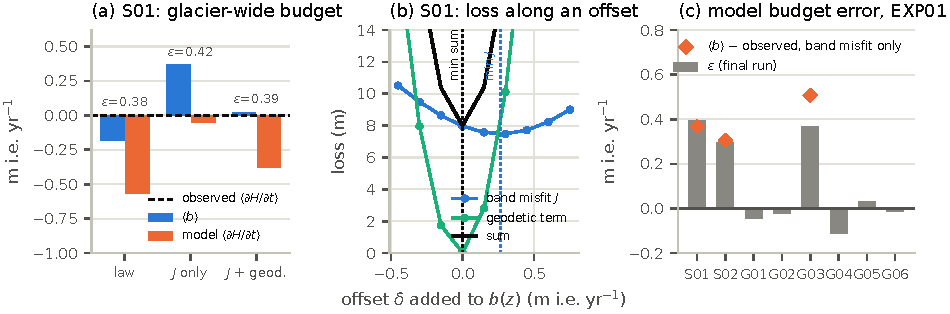
\includegraphics[width=\textwidth]{fig_geod_mechanism.pdf}
\caption{\label{fig:geodmech}How the geodetic term works (EXP01). (a) S01, family means: glacier-wide SMB
$\langle b\rangle$ and modelled mean thickness change over $\Omega$, for the prescribed law, the band misfit $J$ alone and
the final loss; $\varepsilon$ is their difference, Eq.~(\ref{eq:eps}). The observed change is zero. (b) S01,
best-velocity member: the two loss terms and their sum when a uniform offset $\delta$ is added to the final profile
(evaluation runs, no optimisation). (c) Budget error $\varepsilon$ of the final runs on every glacier (bars), and the
departure of $\langle b\rangle$ from the observed change when the inversion uses $J$ alone (diamonds; run for S01, S02 and
G03).}
\end{figure}

The geodetic term and the band misfit complement each other (Fig.~\ref{fig:geodeff}).
\begin{itemize}\setlength{\itemsep}{1pt}
\item \textbf{Cell misfit.} A misfit computed cell by cell is dominated by local errors of the DA thickness, so it
constrains the shape of the profile poorly. On S01 the profile error against the law is
\V{ablCellsRmse}\,\mie\ with it and \V{ablCellsGRmse} with the geodetic term added. The ELA stays at
\V{ablCellsEla}--\V{ablCellsGEla}\,m against the true 2350\,m.
\item \textbf{Band misfit.} It recovers the shape (ELA \V{ablBandsEla}\,m), but it absorbs $\varepsilon$ as a bias of
$\V{ablBandsBias}$\,\mie\ (RMSE \V{ablBandsRmse}).
\item \textbf{Band misfit and geodetic term.} Together they remove the bias ($\V{ablBandsGBias}$) and give the lowest error,
\V{ablBandsGRmse}\,\mie, with an ELA of \V{ablBandsGEla}\,m.
\end{itemize}
The identity has limits. It fails where ice leaves through the outline: at calving fronts, where the glacier is cut by the
domain edge, or where perturbed data put ice outside the real extent (S01 EXP05, Sect.~\ref{sec:s01}). The synthetic
data of S01 do not satisfy it exactly either: the law averages $\V{geodLawNative}$\,\mie\ over the glacier, while the
prescribed d$h$/d$t$ is zero.

\begin{figure}[H]
\centering
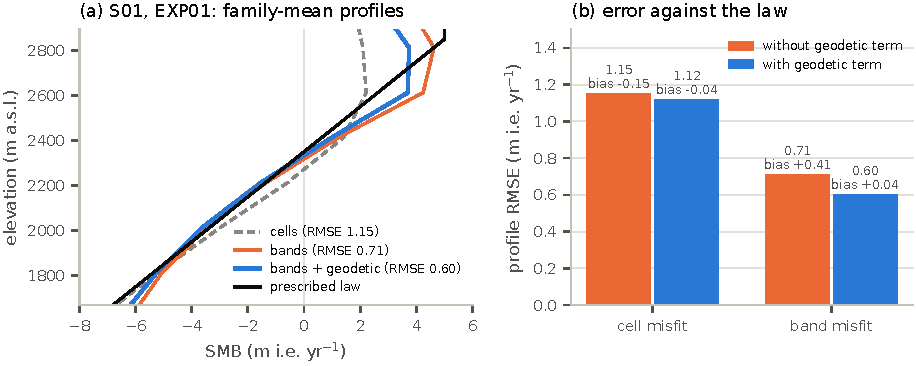
\includegraphics[width=\textwidth]{fig_geod_effect.pdf}
\caption{\label{fig:geodeff}S01, EXP01, with the final forward model and four losses: cell or band misfit, each with and
without the geodetic term. (a) Family-mean profiles against the prescribed law. (b) Profile RMSE against the law, and its
mean bias, over the 1--99\,\% elevation range of the glacier.}
\end{figure}

All results below use the final configuration (band misfit and geodetic term). The first run with the CNN emulator,
which fitted the thickness cell by cell and had no geodetic term, is shown as a reference in Figs.~\ref{fig:loss}
and~\ref{fig:s01} only. For G01 in EXP01 only, the SMB is also inverted as a smooth two-dimensional field instead of a
profile (Sect.~\ref{sec:g01field}).

\begin{table}[!htb]
\centering\small
\caption{ContinuIX experiments (WP2/WP3) and the glaciers run here.}
\label{tab:exp}
\begin{tabular}{lll l}
\toprule
ID & group & content & glaciers \\
\midrule
EXP01 & REF & homogenised, gap-filled data & G01--G06, S01, S02 \\
EXP02 & RAW & raw observations (gaps, several epochs, GPR points) & G01--G06, S02 \\
EXP03--07 & THK & perturbed thickness & G01, G05, S01, S02 \\
EXP08--13 & VEL & perturbed surface velocity & G01, G05, S01, S02 \\
EXP14--15 & RES & changed spatial resolution & G01, G05, S01, S02 \\
EXP16--20 & GLOB & globally available d$h$/d$t$, thickness and velocity products & G01--G06 \\
\bottomrule
\end{tabular}
\end{table}

\begin{table}[!htb]
\centering\small
\caption{Glaciers. Window = inversion period ($t_1$--$t_2$; a 10-yr window is assumed for the synthetic cases);
ice cells on the model grid; ``seg.'' = number of connected GPR profile segments.}
\label{tab:glaciers}
\setlength{\tabcolsep}{4pt}
\begin{tabular}{llrrrrl}
\toprule
 & type & native $\Delta x$ (m) & window (yr) & model $\Delta x$ (m) & ice cells & thickness data \\
\midrule
G01 & ice cap (11 basins) & 25 & 2013--2023 & 100 & 83\,261 & gridded \\
G02 & mountain glacier & 25 & 2006--2013 & 50 & 780 & profiles (10 seg.) \\
G03 & mountain glacier & 20 & 2012--2021 & 100 & 1\,229 & profiles (48 seg.) \\
G04 & mountain glacier & 2 & 2021--2025 & 50 & 887 & gridded \\
G05 & mountain glacier & 10 & 2017.67--2023.64 & 100 & 7\,904 & profiles (147 seg.) \\
G06 & mountain glacier & 10 & 2006--2017 & 100 & 1\,672 & gridded \\
S01 & synthetic, steady state & 1 & 10 yr (assumed) & 50 & 822 & none \\
S02 & synthetic, transient & 100 & 10 yr (assumed) & 100 & 8\,174 & profiles (4 seg.) \\
\bottomrule
\end{tabular}

\end{table}

%=====================================================================================================================
\section{Results}

\subsection{Convergence of the SMB inference}
In the first run the optimisation stopped early. Over all \V{nMemFirst} family members it reduced the loss by a median of
\V{redMedFirst}\,\% in \V{itsMedFirst} L-BFGS iterations, and \V{redBelowFiveFirst}\,\% of the members gained less
than 5\,\%. The final loss keeps decreasing (Fig.~\ref{fig:loss}). Its median reduction is \V{redMedFinal}\,\%
(at least \V{redMinFinal}\,\% for any member), reached in \V{itsMedFinal} iterations. On G05, for example, the
loss falls from \V{lossG05FinalA} to \V{lossG05FinalB}. The two losses measure different things, so their levels
cannot be compared with each other, only their decrease.

\begin{figure}[H]
\centering
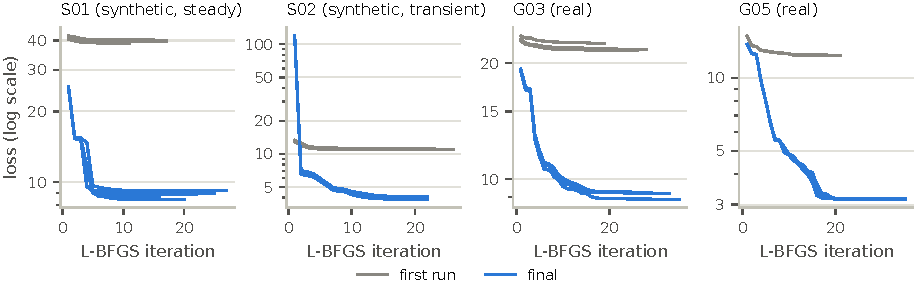
\includegraphics[width=\textwidth]{fig_loss.pdf}
\caption{\label{fig:loss}SMB-inference loss of every family member (EXP01), absolute values on a logarithmic axis.
First run: per-cell RMS thickness misfit at $t_2$ (m) plus curvature penalty. Final: RMS of the band-mean thickness
misfit (m) plus curvature penalty and geodetic term $100\,(\overline{b}-\overline{\Delta H}/\Delta t)^2$. The geodetic
term dominates the first iteration on S02 (\V{lossS02FinalA}).}
\end{figure}

\subsection{S01: comparison with the known SMB}
\label{sec:s01}
S01 is the only glacier with a known SMB, $b(z)=\min[0.01\,(z-2350\,\mathrm{m}),\,5]$\,\mie.
Against this law, the family-mean profile has an RMSE of \V{sOneFinal}\,\mie\ (first run \V{sOneFirst};
Fig.~\ref{fig:s01}a). Cell by cell, the RMSE is \V{sOnePixFinal}\,\mie\ with $R^2=\V{sOneRtwo}$. The members place
the ELA at \V{sOneElaLo}--\V{sOneElaHi}\,m, against a true 2350\,m (first run \V{sOneElaFirstLo}--\V{sOneElaFirstHi}\,m).
The largest deviations, about $\pm1$\,\mie, are in the upper accumulation area. There the profile flattens above
2600\,m instead of rising to the 5\,\mie\ cap.

The final profile is better than the first run in \V{sOneBetter} of the \V{sOneN} S01 experiments
(Fig.~\ref{fig:s01}c), with RMSEs of \V{sOneRegMin}--\V{sOneRegMax}\,\mie\ except in two cases:
\begin{itemize}\setlength{\itemsep}{1pt}
\item \textbf{EXP15} (100\,m grid, on which the glacier is only five cells wide). The error drops from
\V{sOneE15First} to \V{sOneE15Final}\,\mie, but the profile is still far from the law.
\item \textbf{EXP05} is worse (\V{sOneE05First} $\rightarrow$ \V{sOneE05Final}). Its thickness perturbation puts ice
below the real terminus, so the ice mask reaches about 230\,m lower. The geodetic term then follows these
inconsistent data.
\end{itemize}

The remaining error comes with the assimilated state. Without thickness observations, the DA ice is too thick (mean
\V{sOneThk}\,m, against a true \V{sOneThkTrue}\,m). As a result, the modelled glacier is not in balance (Sect.~\ref{sec:geod}): its mean
d$h$/d$t$ is $\V{sOneDhMod}$\,\myr\ (first run $\V{sOneDhModFirst}$), and FDIV has an RMSE of
\V{sOneFdivRmse}\,\mie\ (first run \V{sOneFdivRmseFirst}).

\begin{figure}[H]
\centering
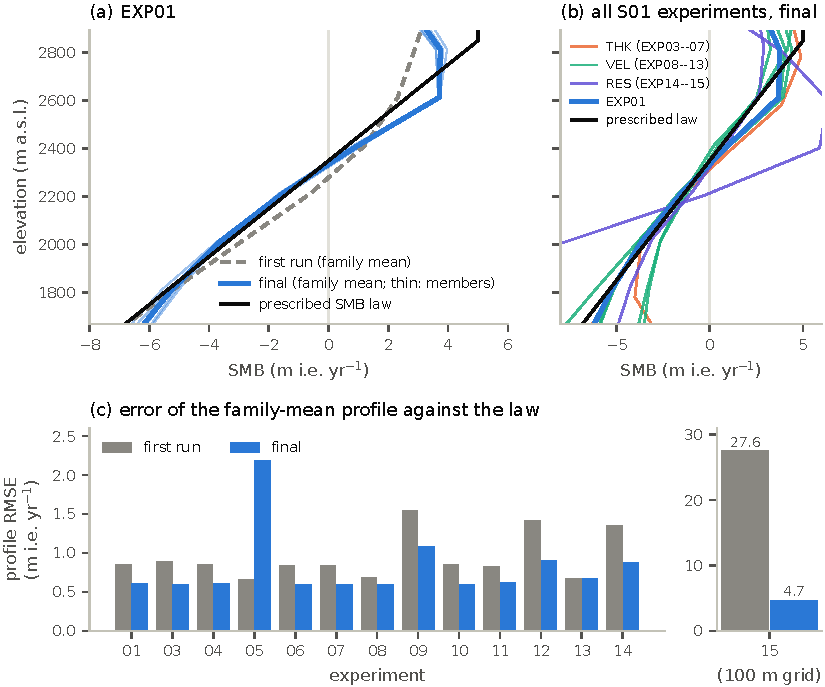
\includegraphics[width=\textwidth]{fig_s01.pdf}
\caption{\label{fig:s01}S01. (a) EXP01: family-mean SMB profile of the final and of the first run, and the prescribed
law. (b) Final family-mean profiles of all S01 experiments; the line leaving the panel is EXP15 (100\,m grid).
(c) RMSE of the family-mean profile against the law, over the glacier's 1--99\,\% elevation range; EXP15 on its own scale.}
\end{figure}

\subsection{S02: thickness and sensitivity of the SMB}
S02 comes with its true thickness but without an SMB field. The assimilated thickness has a bias of $\V{sTwoThkBias}$\,m
and an RMSE of \V{sTwoThkRmse}\,m ($r=\V{sTwoThkR}$; Fig.~\ref{fig:s02thk}). It is too thin along the main trunk and
too thick near the margins. The glacier-wide SMB is $\V{sTwoGw}$\,\mie, close to the observed mean d$h$/d$t$
($\V{sTwoDhObs}$\,\myr; first run $\V{sTwoGwFirst}$\,\mie). The modelled thinning is stronger
($\V{sTwoDhMod}$\,\myr), and the ELA is at \V{sTwoEla}\,m.

Across all experiments the glacier-wide SMB stays between $\V{sTwoGwMin}$ and $\V{sTwoGwMax}$\,\mie. This includes the
300\,m grid of EXP14, on which the first run failed. The shape of the profile is less robust (Fig.~\ref{fig:s02prof}),
and its sensitivity depends on the input:
\begin{itemize}\setlength{\itemsep}{1pt}
\item \textbf{GPR thickness} (changed by 13--30\,\%) moves the profile by at most \V{respThkMaxS02}\,\mie, close to
the scatter between runs with identical inputs (\V{repeatFloor}\,\mie).
\item \textbf{Surface velocity} matters more. The +44\,\% speed bias of EXP13 moves the profile by \V{respS02E13}\,\mie\
and raises the ELA to \V{sTwoElaE13}\,m. The noise of EXP09 moves it by \V{respS02E09}\,\mie.
\item \textbf{Resolution.} The 300\,m grid (EXP14) moves the profile by \V{respS02E14}\,\mie.
\item \textbf{Raw data} (EXP02) move it by \V{respS02E02}\,\mie, because the raw velocities cover only the lower
33\,\% of the glacier. The ELA drops to \V{sTwoElaE02}\,m.
\end{itemize}

\begin{figure}[H]
\centering
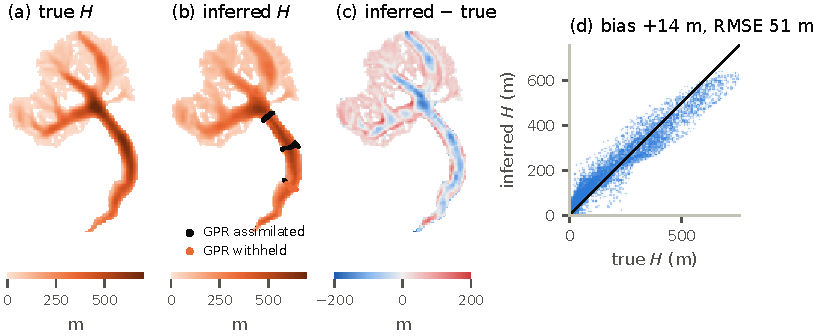
\includegraphics[width=\textwidth]{fig_s02_thickness.pdf}
\caption{\label{fig:s02thk}S02, EXP01: (a) true and (b) inferred thickness with the assimilated and withheld GPR cells,
(c) difference, (d) cell-by-cell comparison.}
\end{figure}

\begin{figure}[H]
\centering
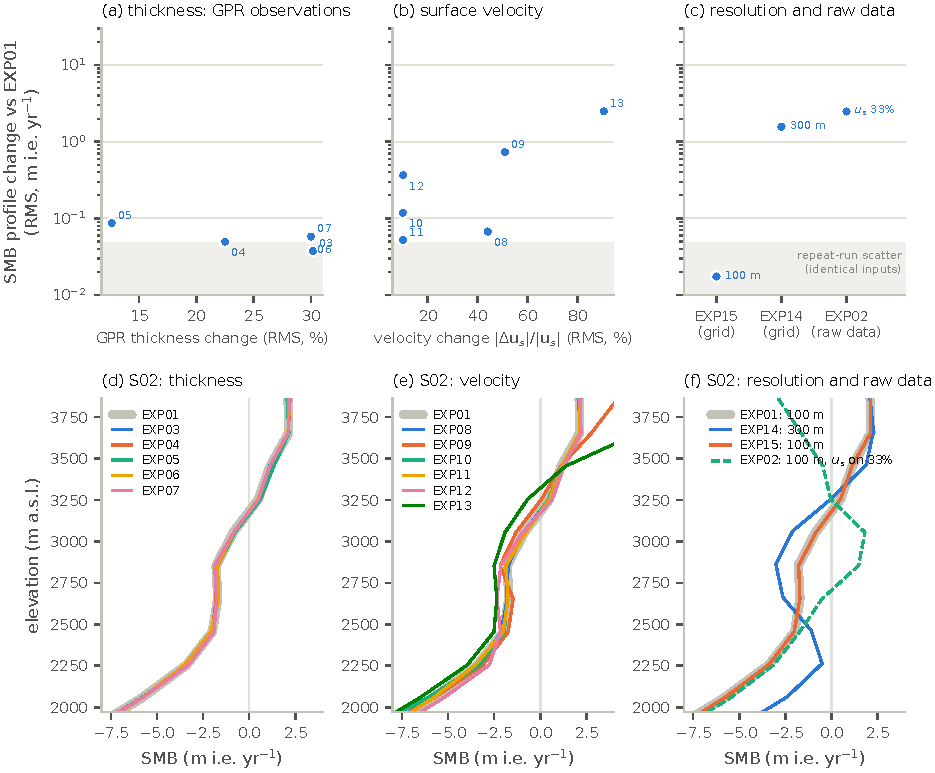
\includegraphics[width=\textwidth]{fig_s02_profiles.pdf}
\caption{\label{fig:s02prof}S02, sensitivity to the inputs. Top: change of the input that reaches the method, against
the RMS change of the SMB profile relative to EXP01 (numbers = experiment). The grey band is the scatter between runs
with identical inputs. Bottom: family-mean profiles, with EXP01 as the wide grey line.}
\end{figure}

\subsection{Real glaciers, EXP01}
Figure~\ref{fig:real} shows the SMB profiles of the six real glaciers, and Fig.~\ref{fig:g05} gives the fields of G05.
The modelled mean d$h$/d$t$ (\myr) compares with the observed one as follows:
G01 $\V{dhModG01}$ against $\V{dhObsG01}$, G02 $\V{dhModG02}$ against $\V{dhObsG02}$, G03 $\V{dhModG03}$ against
$\V{dhObsG03}$, G04 $\V{dhModG04}$ against $\V{dhObsG04}$, G05 $\V{dhModG05}$ against $\V{dhObsG05}$, and G06
$\V{dhModG06}$ against $\V{dhObsG06}$.
The two agree closely on G01, G05 and G06. The modelled thinning is too strong on G03 and too weak on G04, and on
G02 the modelled thickening is too weak. The positive d$h$/d$t$ of G02 is doubtful and remains an open question to the
organisers.

Where independent GPR profiles exist, the RMS thickness misfit to them is \V{gprTestG02}\,m (G02),
\V{gprTestG03}\,m (G03) and \V{gprTestG05}\,m (G05). The mean $\sigma_{\rm SMB}$ ranges from \V{uncMin} to
\V{uncMax}\,\mie. It is almost entirely the residual within 50\,m elevation bands, i.e.\ the part of the thickness
change that a profile $b(z)$ cannot represent. The spread between family members adds at most \V{famSpreadMax}\,\mie.

\begin{figure}[H]
\centering
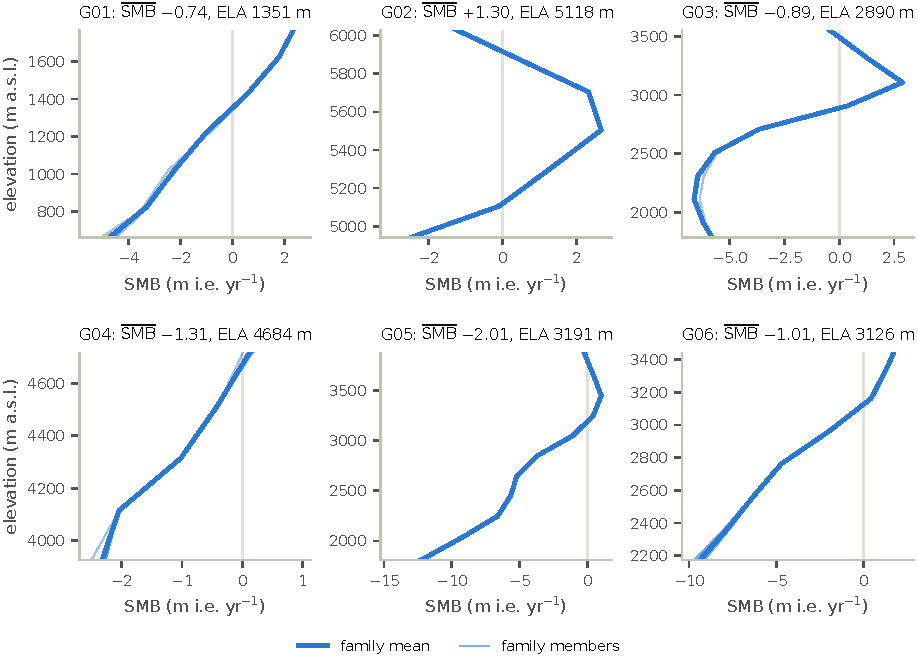
\includegraphics[width=\textwidth]{fig_real_profiles.pdf}
\caption{\label{fig:real}Real glaciers, EXP01: SMB profiles of the family members and their mean. The titles give the
glacier-wide SMB (\mie) and the family-mean ELA.}
\end{figure}

\begin{figure}[H]
\centering
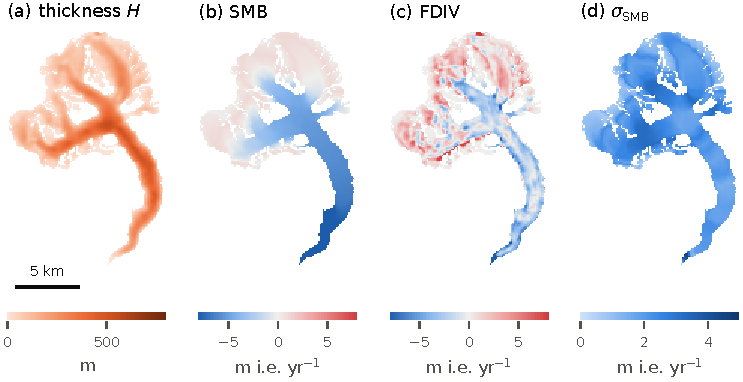
\includegraphics[width=\textwidth]{fig_g05_maps.pdf}
\caption{\label{fig:g05}G05, EXP01 (native grid): (a) assimilated thickness, (b) SMB, (c) flux divergence, (d) SMB
uncertainty.}
\end{figure}

\subsection{G01, EXP01: two-dimensional SMB field}
\label{sec:g01field}
On the G01 ice cap a single profile $b(z)$ cannot represent the SMB differences between the basins. For EXP01 only, we
therefore also invert the SMB as a field $b(x,y)$. The field is static over the window, and it is bilinear between
nodes \V{fldNodes}\,m apart, so no detail below that scale can be fitted. The loss is the cell-by-cell RMS thickness
misfit at the end of the window. It also contains the geodetic term and a smoothness penalty, which is
$\lambda$ times the mean squared gradient between nodes. Each family member starts from its own profile solution. All
other settings are those of the profile inversion.

We chose $\lambda=\V{fldReg}$ at the corner of the L-curve (Fig.~\ref{fig:g01field}f). Below $\lambda=1$ the field
breaks up into patches that fit noise in the thickness change. Over the \V{fldN} family members the 2-D field gives the following results:
\begin{itemize}\setlength{\itemsep}{1pt}
\item \textbf{Misfit.} The RMS cell misfit falls from \V{fldCellProf} to \V{fldCellField}\,m, and the RMS of the
50\,m band means falls from \V{fldBandProf} to \V{fldBandField}\,m. The field therefore also fits the band means
better than the profile, even though the profile was fitted to exactly those means.
\item \textbf{Glacier-wide SMB and ELA.} The glacier-wide SMB changes from $\V{fldGwProf}$ to $\V{fldGwField}$\,\mie;
both are set by the geodetic term. The modelled mean d$h$/d$t$ is $\V{fldDhField}$, against $\V{fldDhObs}$\,\myr\
observed. The ELA of the mean profile of the field over elevation is \V{fldElaField}\,m, against \V{fldElaProf}\,m.
\item \textbf{Spatial pattern.} The field departs from the profile by up to \V{fldDiffMax}\,\mie\ (95th percentile).
It has more accumulation in the western interior and stronger ablation on several outlet lobes, at the same
elevation (Fig.~\ref{fig:g01field}c).
\item \textbf{Uncertainty.} $\sigma_{\rm SMB}$ drops from \V{fldUncProf} to \V{fldUncField}\,\mie, because less of
the thickness change remains unexplained.
\end{itemize}
G01 has no known SMB, so these results show a better fit to the data, not a validated improvement in accuracy. All
other sections, including G01 under perturbation, use the profile.

\begin{figure}[H]
\centering
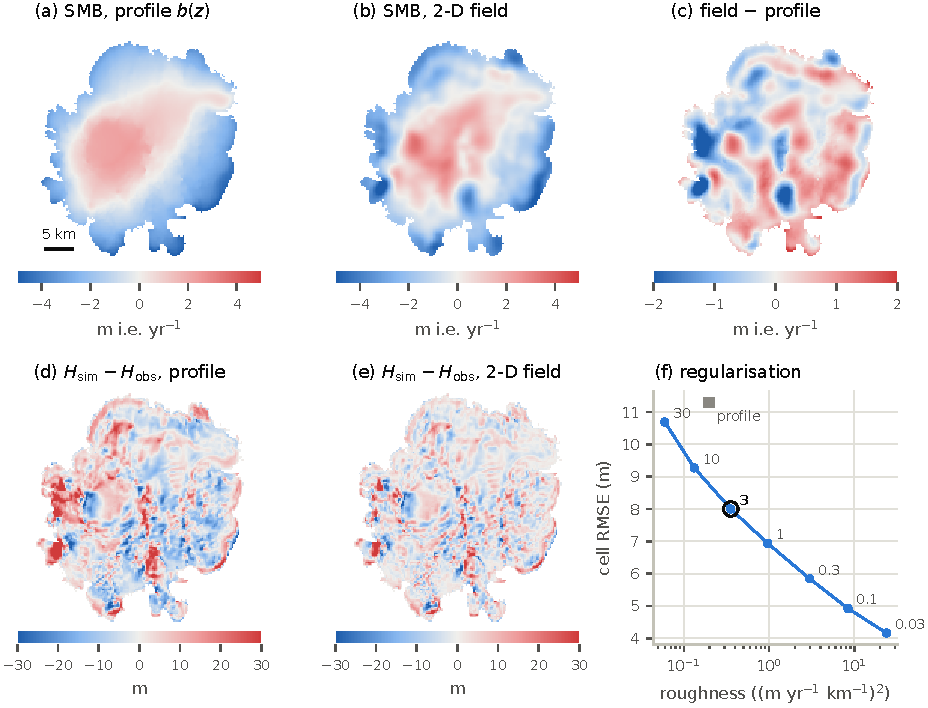
\includegraphics[width=\textwidth]{fig_g01_field.pdf}
\caption{\label{fig:g01field}G01, EXP01: SMB as a 2-D field ($\lambda=\V{fldReg}$, \V{fldNodes}\,m nodes)
against the profile $b(z)$. (a, b) Family-mean SMB on the native grid and (c) their difference. (d, e)
End-of-window thickness misfit of the best-velocity member on the model grid. (f) L-curve for that member: cell
misfit against field roughness for $\lambda$ from 0.03 to 30 (labels). The square marks the profile solution
evaluated on the node grid.}
\end{figure}

\subsection{G01 and G05 under perturbation}
The glacier-wide SMB does not respond to the thickness and velocity perturbations (EXP03--13). It changes by at most
\V{dSmbMaxNoResG05}\,\mie\ on G05 and \V{dSmbMaxNoResG01} on G01. It moves only on the coarser grids of G05,
because the observed mean d$h$/d$t$ itself changes there: on EXP14 the SMB is $\V{gwG05EXP14}$ for a d$h$/d$t$ of
$\V{dhG05EXP14}$, and on EXP15 $\V{gwG05EXP15}$ for $\V{dhG05EXP15}$, against $\V{gwG05}$ in EXP01. The ELA stays
within \V{dElaMaxG01}\,m of EXP01 on G01 and within \V{dElaMaxG05}\,m on G05; the largest shift is under the speed bias
of EXP13 on both glaciers.

The shape of the profile responds more (Fig.~\ref{fig:realexpprof}):
\begin{itemize}\setlength{\itemsep}{1pt}
\item \textbf{G01.} Only EXP13 moves the profile clearly beyond the repeat-run scatter (\V{respG01E13}\,\mie).
\item \textbf{G05.} The 100\,m grid of EXP15 moves it most (\V{respG05E15}\,\mie), followed by the perturbed GPR
thickness (up to \V{respThkMaxG05}\,\mie) and EXP14 (\V{respG05E14}). The velocity perturbations stay below
\V{respVelMaxG05}\,\mie.
\item \textbf{Raw data} (EXP02) reproduce EXP01 on both glaciers. The glacier-wide SMB is $\V{rawGwG01}$ on G01 and
$\V{rawGwG05}$\,\mie\ on G05, and the ELA moves by \V{rawElaG01} and \V{rawElaG05}\,m.
\end{itemize}

\begin{figure}[H]
\centering
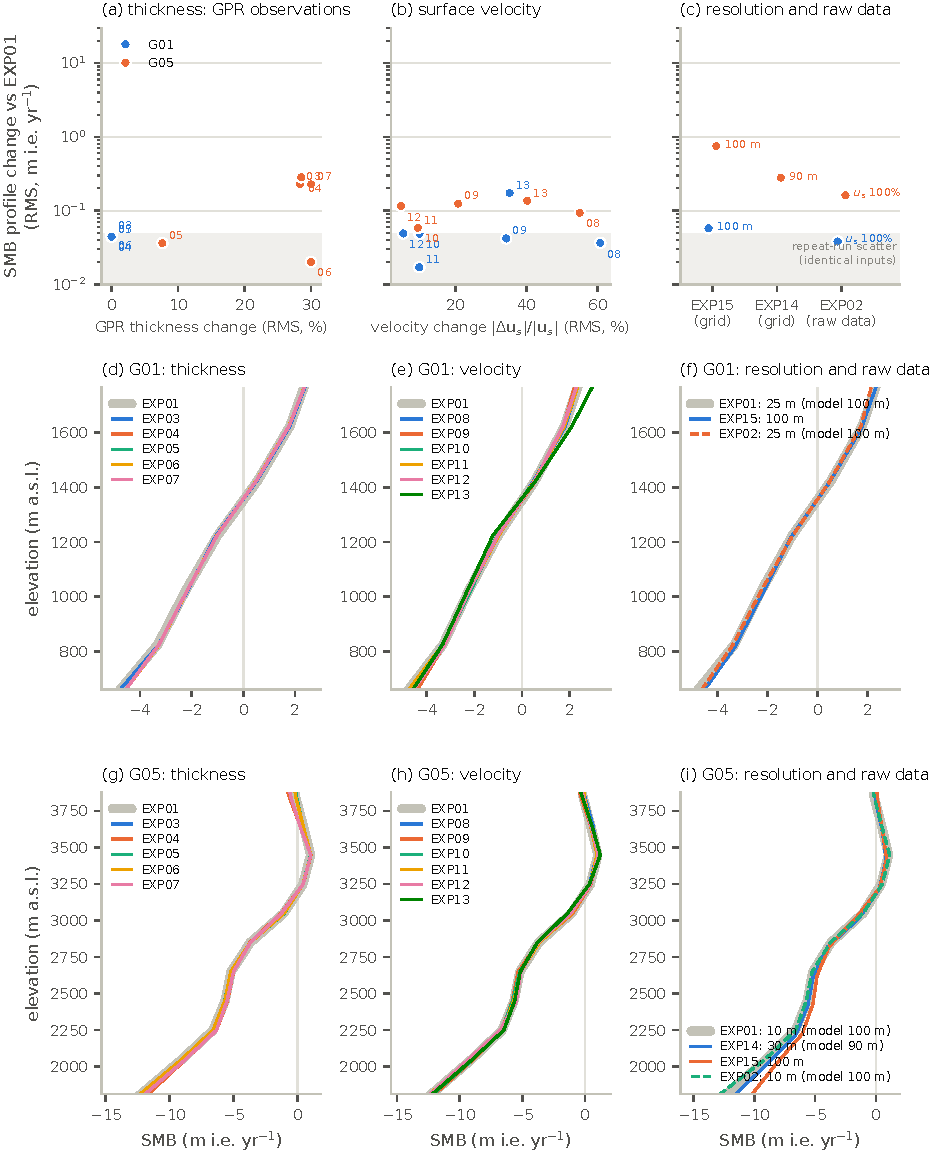
\includegraphics[width=\textwidth]{fig_real_exp_profiles.pdf}
\caption{\label{fig:realexpprof}G01 and G05, sensitivity to the inputs, as in Fig.~\ref{fig:s02prof}. G01 has no GPR, so
its thickness experiments are repeats of EXP01 and are plotted at zero change. Rows 2--3: family-mean profiles of every
experiment, with EXP01 as the wide grey line; the legends give the native and model grid spacing.}
\end{figure}

\subsection{Raw data and globally available inputs}
On all six real glaciers the raw data (EXP02) keep the glacier-wide SMB within \V{rawGwMax}\,\mie\ of EXP01 and the
ELA within \V{rawElaMax}\,m (Fig.~\ref{fig:glob}). This holds even where the inferred thickness drops, as on G04
(\V{glThkG04E01} $\rightarrow$ \V{glThkG04E02}\,m) and G06 (\V{glThkG06E01} $\rightarrow$ \V{glThkG06E02}\,m).

The global experiments (EXP16--20) all use the 2000--2020 elevation change of \citet{hugonnet}. The main effects are:
\begin{itemize}\setlength{\itemsep}{1pt}
\item \textbf{The glacier-wide SMB follows that product} (EXP01 $\rightarrow$ EXP17, in \mie): G01
$\V{glG01E01}\rightarrow\V{glG01E17}$, G02 $\V{glG02E01}\rightarrow\V{glG02E17}$, G03 $\V{glG03E01}\rightarrow\V{glG03E17}$,
G04 $\V{glG04E01}\rightarrow\V{glG04E17}$, G05 $\V{glG05E01}\rightarrow\V{glG05E17}$, G06
$\V{glG06E01}\rightarrow\V{glG06E17}$. On G02 the site and global elevation changes disagree in sign.
\item \textbf{The global velocities} of \citet{millan} (EXP16, EXP20) change the inferred thickness strongly. On G01 it
rises from \V{glThkG01E01} to \V{glThkG01E16}--\V{glThkG01E20}\,m, on G06 it falls from \V{glThkG06E01} to
\V{glThkG06E16}\,m, and on G04 from \V{glThkG04E01} to \V{glThkG04E16}\,m. With these velocities the G06 profile no
longer crosses zero on the glacier, so there is no ELA. The same happens on G04 with the site velocities (EXP17--19).
\item \textbf{Repeatability.} Some runs have identical inputs for our method: EXP17--19 everywhere, and EXP16 and
EXP20 on G01, G04 and G06. They still differ through the L-curve choice of the regularisation, which changes the mean
thickness by up to \V{idThkMax}\,m. Their glacier-wide SMB, however, agrees to better than 0.01\,\mie, and their ELA to
within \V{idElaMax}\,m.
\item \textbf{Uncertainty.} $\sigma_{\rm SMB}$ is \V{uncRatioMin} to \V{uncRatioMax} times its EXP01 value.
\end{itemize}

\begin{figure}[H]
\centering
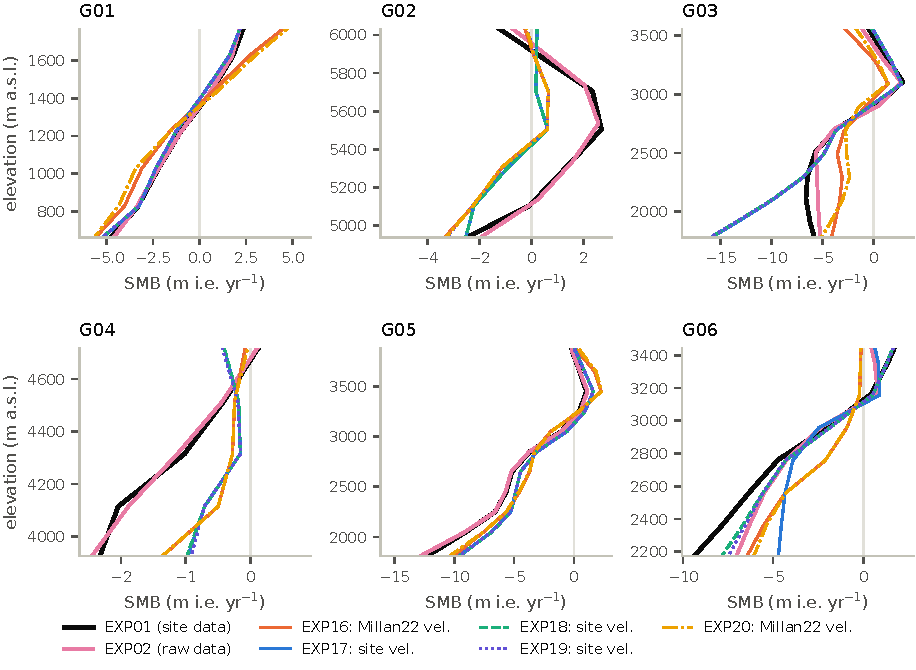
\includegraphics[width=\textwidth]{fig_glob_profiles.pdf}
\caption{\label{fig:glob}Real glaciers: family-mean SMB profiles with site data (EXP01), raw data (EXP02) and globally
available inputs (EXP16--20). EXP17--19 have identical inputs for our method, as have EXP16 and EXP20 on G01, G04 and G06.}
\end{figure}

%=====================================================================================================================
\section{Summary}
\begin{itemize}\setlength{\itemsep}{1pt}
\item The final SMB inference converges. The median loss reduction is \V{redMedFinal}\,\%, against \V{redMedFirst}\,\%
in the first run.
\item On S01 the profile error against the known SMB is \V{sOneFinal}\,\mie\ (first run \V{sOneFirst}), and the ELA is
\V{sOneElaLo}--\V{sOneElaHi}\,m against 2350\,m. The final run is better in \V{sOneBetter} of \V{sOneN} experiments and
worse in \V{sOneWorse}, whose perturbed thickness is inconsistent with the glacier extent.
\item The glacier-wide SMB is tied to the observed elevation change. It is therefore robust to the perturbations, to the
raw data and to the choice of regularisation, and it follows the global d$h$/d$t$ product when that product is used.
\item On G01 (EXP01), a smooth 2-D SMB field reduces the cell misfit from \V{fldCellProf} to \V{fldCellField}\,m
and $\sigma_{\rm SMB}$ from \V{fldUncProf} to \V{fldUncField}\,\mie, and the glacier-wide SMB stays at $\V{fldGwField}$\,\mie.
\item The shape of the profile is most sensitive to the surface velocity (bias, coverage of the raw data) and to the
grid spacing, and least sensitive to the GPR thickness.
\item Open points: the DA thickness where no GPR exists (S01: mean \V{sOneThk}\,m against a true \V{sOneThkTrue}\,m,
which biases FDIV), the missing EXP14 for G01, and the sign of the G02 elevation change.
\end{itemize}

\begin{thebibliography}{99}\small
\bibitem[ContinuIX(2026)]{continuix} ContinuIX working group: Protocol for work packages 2 and 3, \url{https://github.com/ContinuIX/ContinuIX-1}; data: \url{https://doi.org/10.5281/zenodo.21401808}, 2026.
\bibitem[Jouvet et al.(2026)]{igm} Jouvet, G., Finley, B., Gregov, T., and Rosier, S.: IGM: an accessible, modular, differentiable, and GPU-accelerated high-order ice flow model, EarthArXiv, \url{https://doi.org/10.31223/X5GB6G}, 2026.
\bibitem[Lleshi et al.(submitted)]{lleshi} Lleshi, K., Jouvet, G., Kneib, M., Gregov, T., and Herman, F.: Surface mass balance inference based on a transient glacier evolution model inversion, The Cryosphere, submitted.
\bibitem[Hugonnet et al.(2021)]{hugonnet} Hugonnet, R., McNabb, R., Berthier, E., et al.: Accelerated global glacier mass loss in the early twenty-first century, Nature, 592, 726--731, 2021.
\bibitem[Millan et al.(2022)]{millan} Millan, R., Mouginot, J., Rabatel, A., and Morlighem, M.: Ice velocity and thickness of the world's glaciers, Nat. Geosci., 15, 124--129, 2022.
\end{thebibliography}

\end{document}
